%!TEX root = skripsi.tex
%-----------------------------------------------------------------------------%
\chapter{\babTiga}
%-----------------------------------------------------------------------------%
Bab ini akan menjelaskan gambaran proses penelitian secara keseluruhan mulai dari rancangan sistem sampai dengan metode evaluasi. Rancangan dari sistem mempunyai dua hasil utama yaitu \textit{sense tagged corpus} dan sistem WSD Bahasa Indonesia.

\section{Rancangan Sistem}

Rancangan sistem pada penelitian ini dapat dilihat pada gambar \ref{fig:Rancangan-Sistem} berikut.

\begin{figure}
	\centering
	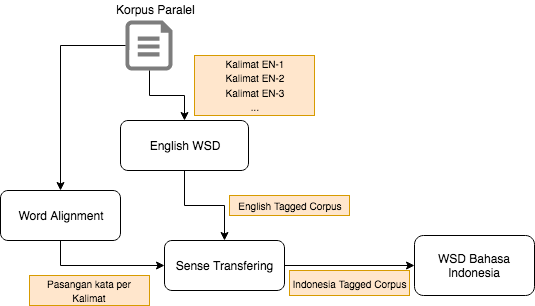
\includegraphics[width=1\linewidth]{adit_pics/WSD-full.png}
	\caption{Rancangan Sistem}
	\label{fig:Rancangan-Sistem}
\end{figure}

Proses \textit{pipeline} terdiri dari pembuatan \textit{sense tagged corpus} bahasa Inggris,  \textit{word alignment} korpus paralel, peningkatan kualitas dan evaluasi \textit{word alignment}, pemindahan \textit{sense} dari korpus bahasa Inggris, dan sistem WSD yang diimplementasikan. Semua data di dalam korpus Identic digunakan dalam proses \textit{word alignment} dan \textit{English} WSD di atas.
%-----------------------------------------------------------------------------%

\section{Pembangunan \textit{Sense Tagged Corpus} Bahasa Inggris}
%-----------------------------------------------------------------------------%

Pembangunan \textit{sense tagged corpus} bahasa Inggris dilakukan dengan menggunakan \textit{tool} IMS \citep{zhong2010makes} untuk mendapatkan makna terbaik yang dapat ditag oleh \textit{tool} tersebut. Makna kata hasil dari proses ini akan dipindahkan ke kata yang bersesuaian pada kalimat yang sama pada bagian \textit{sense transfering}. Gambaran proses secara singkat dapat dilihat pada \ref{fig:producing-en-tag-corpus} berikut.


\begin{figure}
	\centering
	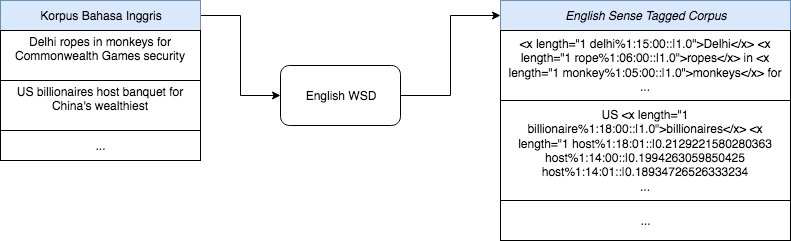
\includegraphics[width=1\linewidth]{adit_pics/bab-3-en-tag-corpus.png}
	\caption{Ilustrasi Pembuatan \textit{sense tagged corpus} Bahasa Inggris}
	\label{fig:producing-en-tag-corpus}
\end{figure}

\textit{File} yang diberikan sebagai masukan dari IMS adalah korpus Bahasa Inggris yang berisi kalimat-kalimat  dalam Bahasa Inggris. Korpus ini didapatkan setelah memisahkan konten dari korpus Identic menjadi dua buah korpus Bahasa Indonesia dan Bahasa Inggris. Keluaran dari proses ini adalah korpus berbahasa Inggris dengan kata-kata yang sudah diberikan \textit{tag} berupa \textit{sense key} yang memungkinkan untuk kata tersebut. Hasil tersebut kemudian akan diproses lagi untuk memilih \textit{sense} terbaik dan menyederhanakan format untuk proses berikutnya yang akan dijelaskan lebih rinci pada bab implementasi.
%-----------------------------------------------------------------------------%
\section{\textit{Word Alignment} Bahasa Indonesia - Bahasa Inggris}
%-----------------------------------------------------------------------------%

Korpus utama yang digunakan sebagai sumber data penelitian ini adalah korpus Identic \citep{larasati2012identic}. Korpus identik berisi pasangan kalimat-kalimat dalam bahasa Indonesia dan Inggris. Kalimat yang berpasangan di dalamnya sebagian besar mempunyai makna konten yang paralel walaupun terdapat juga yang \textit{comparable}. Korpus identik ini mempunyai total sebanyak 88.918 buah pasangan kalimat di dalamnya. Format korpus Identic adalah sebagai berikut:
\begin{lstlisting}
<ID><tab><Kalimat Indonesia><tab><Kalimat Inggris>
\end{lstlisting}
\clearpage
Contoh isi dari korpus Identic yang digunakan berbentuk seperti berikut ini:
\begin{lstlisting}[backgroundcolor = \color{white}]
...
panl-bppt-eco-s1505	Ada 10 sektor yang dibicarakan.	There are 10 sectors that have been on the talk.
panl-bppt-eco-s1508	Semua ketentuan Insya Allah akan selesai 1 April, kata Burhanuddin.	All the regulations, God willing, will be completed on April 1, he said.
...
\end{lstlisting}


Proses \textit{word alignment} ini dilakukan agar nantinya makna kata dari suatu kata dalam Bahasa Inggris dapat ditransfer ke kata yang bersesuaian pada Bahasa Indonesia. Gambaran proses dapat dilihat pada gambar \ref{fig:giza-aligning}.

\begin{figure}
	\centering
	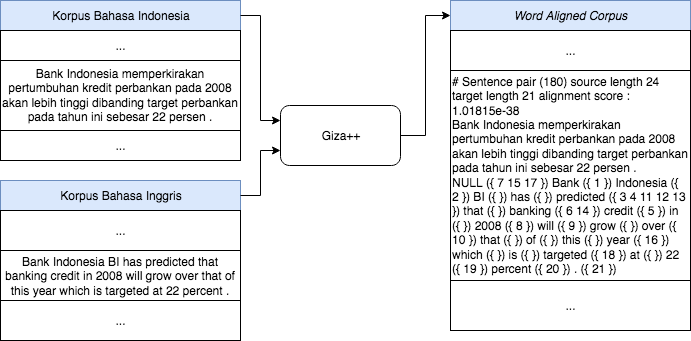
\includegraphics[width=1\linewidth]{adit_pics/giza-process.png}
	\caption{Ilustrasi \textit{alignment} dengan Giza++}
	\label{fig:giza-aligning}
\end{figure}

Penjelasan dair proses \textit{alignment} tersebut meliputi tahap-tahap berikut:
\begin{enumerate}
	\item Mempersiapkan kedua buah \textit{file} yaitu korpus bahasa asal (\textit{source}) dan korpus bahasa tujuan (\textit{target}). Kedua \textit{file} ini berpasangan dalam setiap barisnya. Baris pertama dalam \textit{file} pertama berpasangan dengan baris pertama pada \textit{file} kedua sampai akhir baris pada kedua \textit{file}.
	\item Menghasilkan \textit{file} perbendaharaan kata dari kedua bahasa dan \textit{list} indeks perbendaharaan kata pada tiap kalimat yang sudah diselaraskan
	\item Menghasilkan \textit{cooccurence file} dari kosa kata dan pasangan kalimat tersebut
	\item Proses \textit{alignment} yang menghasilkan beberapa macam \textit{output file} 
\end{enumerate}

Terdapat satu buah \textit{output file} Giza++ yang berisi pasangan-pasangan kalimat dengan kata-kata yang sudah diselaraskan dengan translasinya dalam bahasa tujuan. Hasil ini merupakan \textit{best viterbi alignment} menurut Giza++. Penjelasan lebih mendalam tentang \textit{output file} Giza++ tersebut akan dibahas pada bab implementasi. Hasil dari proses ini kemudian akan ditingkatkan kualitasnya sebelum melakukan proses \textit{sense transfering}.

Proses peningkatan kualitas hasil alignment diperlukan untuk meminimalisasi kesalahan pemasangan kata-kata pada proses sebelumnya. Permasalahan  yang terjadi adalah adanya pasangan-pasangan kata yang tidak benar seperti pada halnya kata "lapangan" misalnya yang  dipasangkan dengan kata dalam bahasa Inggris yaitu \textit{field}, \textit{ground}, \textit{involved}, \textit{job}, \textit{program}, dan beberapa kata lainnya. Peningkatan kualitas \textit{alignment} ini dilakukan dengan dua buah pendekatan, yaitu dengan bantuan \textit{online dictionary} bahasa Indonesia-Inggris dan \textit{bi-directional alignment}. 

Pendekatan dengan bantuan kamus \textit{online} diterapkan dengan mencari kata terjemahan pada bahasa Inggris dari suatu kata dalam Bahasa Indonesia untuk menentukan apakah \textit{alignment} benar atau salah. Pada pendekatan kedua, dilakukan \textit{inverse} \textit{alignment} antara bahasa Indonesia ke Inggris (\textit{bi-directional}). Jika pada proses awal \textit{alignment} dilakukan dengan menerapkan bahasa Indonesia sebagai \textit{source} dan Inggris sebagai \textit{target}, kali ini dilakukan proses yang berkebalikan. Gambaran proses secara umum pada \textit{bi-directional} ini dapat dilihat pada gambar \ref{fig:Bidirectional-Enhancement}.

\begin{figure}
	\centering
	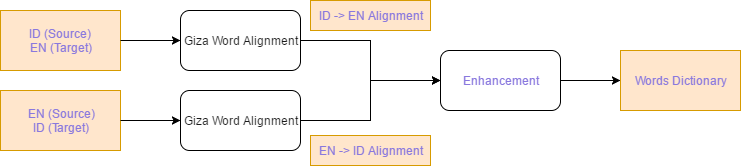
\includegraphics[width=1\linewidth]{adit_pics/bidirectional-enhancement.png}
	\caption{Bi-directional \textit{word alignment}}
	\label{fig:Bidirectional-Enhancement}
\end{figure}


Pemanfaatkan hasil \textit{alignment} korpus bahasa Inggris ke Indonesia akan menghasilkan pasangan-pasangan kata dengan tingkat kesalahan \textit{alignment} lebih kecil dari \textit{alignment} satu arah saja. Metode yang akan dilakukan adalah dengan memeriksa setiap pasangan kata dari bahasa Indonesia yang mana merupakan kata dalam bahasa Inggris, apakah kata tersebut memiliki pasangan dalam \textit{inverse alignment} Giza.




%-----------------------------------------------------------------------------%
\section{\textit{Sense Transfering}} \label{sec:Sense Transfering}
%-----------------------------------------------------------------------------%
Pemindahan makna kata dilakukan dengan beberapa \textit{sub-process} yang terdiri dari pemasangan antar kalimat, pemeriksaan kata, dan \textit{sense transfering}.
\begin{enumerate}
	\item Pemasangan antar kalimat yang bersesuaian dengan kata-kata yang berpasangan. Pada contoh kata "halaman" yang berpasangan dengan "courtyard", maka pasangan kalimat "Aku bermain di halaman" akan dipasangkan dengan kalimat "I play at the courtyard". Pemeriksaan untuk kata yang saling berpasangan menggunakan hasil dari \textit{alignment} dan kamus hasil \textit{alignment enhancement}.
	\item \textit{Sense} dari kata yang menjadi \textit{target} tersebut ("halaman") kemudian diperiksa dengan \textit{sense} kata yang sama yang sudah pernah dipindahkan dari pasangan kalimat lain. Jika \textit{sense} yang ingin dipindahkan "mirip" dan memiliki kedekatan makna di atas batas \textit{threshold}, maka \textit{sense} yang akan dipindahkan hanya salah satunya saja. Proses ini diperlukan untuk meminimalisasi adanya satu kata bahasa Indonesia yang mempunyai lebih dari satu \textit{sense} yang mirip dari definisi makna tersebut.
	\item Pemindahan makna dilakukan sebagai proses akhir. Bila "courtyard" memiliki \textit{sense} yang artinya adalah "pekarangan rumah", maka "halaman" pada kalimat "Aku bermain di halaman" memiliki \textit{sense} "pekarangan rumah".
\end{enumerate}

\section{WSD Bahasa Indonesia} \label{sec:Sistem WSD}
%-----------------------------------------------------------------------------%
Sistem WSD yang dibangun adalah dengan menggunakan pendekatan \textit{supervised learning}. \textit{Classifier} yang digunakan dalam sistem \textit{WSD} ini adalah SVM dengan fitur-fitur tertentu. Pengujian dilakukan dengan menggunakan beberapa fitur seperti \textit{bag of words}, \textit{POS Tag}, dan \textit{word embedding}. Fitur \textit{bag of words} menggunakan \textit{window} sebanyak dua buah kata kanan dan kiri kata tujuan sebagai kata konteks. Fitur \textit{POS Tag} dan vektor \textit{word embedding} juga akan dicoba sebagai skenario pada penelitian ini. Pada ekstraksi fitur, kata-kata yang termasuk dalam stopwords \citep{tala2003study} tidak digunakan sebagai fitur.

Fitur \textit{bag of words} menggunakan pendekatan kemunculan kata-kata pada konteks kalimat sebagai fitur. Kata yang diambil untuk dijadikan fitur adalah dua buah kata di kiri dan di kanan dari \textit{target word}. Proses diawali dengan mencari \textit{target word} pada kalimat, kemudian ambil kata sebelum dan sesudah dari \textit{target word} tersebut. Contoh dari fitur ini dapat dilihat pada kalimat dengan \textit{target word} "bisa" berikut.
\begin{lstlisting}[backgroundcolor = \color{white}]
Ani digigit ular dengan bisa yang berbahaya
\end{lstlisting}
Pada contoh kalimat tersebut, \textit{bag of words} yang diambil adalah "digigit", "ular", dan "berbahaya". Kata "yang" tidak masuk sebagai fitur karena termasuk dalam stopwords. Jika misalkan kata-kata keseluruhan dari \textit{context window} tersebut misalnya ["digigit", "ular", "makan", "berbahaya", "akrobat"], maka vektor fitur \textit{bag of words} dari kalimat tersebut adalah [1,1,0,1,0].

Setiap fitur \textit{bag of words} dari setiap kalimat tersebut dikumpulkan untuk menjadi satu fitur besar yang mendeteksi kemunculan kata-kata tersebut pada setiap kalimat.

Pada fitur POS Tag kelas kata yang diambil adalah POS Tag dari \textit{target word} kata sebelum, dan kata sesudahnya. Kelas kata dari \textit{target word} diperhitungkan karena pada beberapa kasus kata polisemi dapat dibedakan maknanya berdasarkan POS Tag yang dimilikinya. Kelas pada POS Tag yang digunakan meliputi NN(Noun), NNP(Proper Noun), VB(verb), CC(Coordinating conjunction), dan lain-lain. Pembentukan kelas POS Tag untuk menjadi fitur dilakukan dengan proses yang serupa pada fitur \textit{bag of words} di mana kombinasi kombinasi dari POS Tag yang mungkin direpresentasikan dalam \textit{one hot representation}. Hal ini dapat diilustrasikan dengan proses berikut:

\begin{enumerate}
	\item Simpan POS Tag dari indeks kata masing-masing (\textit{target word}-1, \textit{target word}, \textit{target word}+1)
	\item Untuk masing-masing indeks baik itu -1,0,dan 1
	\item Kumpulkan POS Tag yang \textit{distinct}, populasikan dalam \textit{array}
	\item \textit{Array} ini nantinya akan merepresentasikan keberadaan POS Tag tertentu pada kata dengan indeks terkait tersebut
\end{enumerate}

Pada fitur \textit{word embedding}, vektor yang dijadikan sebagai fitur adalah vektor dari semua kata pada kalimat tersebut. Proses tersebut dapat diilustrasikan pada gambar \ref{fig:Ilustrasi-Fitur-Word-Embedding}.
\begin{figure}
	\centering
	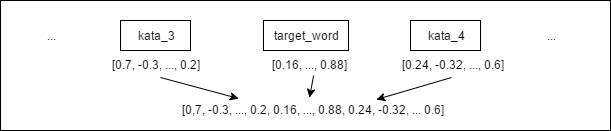
\includegraphics[width=1\linewidth]{adit_pics/we-vector.png}
	\caption{Ilustrasi Fitur Word Embedding}
	\label{fig:Ilustrasi-Fitur-Word-Embedding}
\end{figure}

Semua vektor nilai dari kata-kata tersebut kemudian dikonkatenasi menjadi satu buah vektor besar. Untuk menjamin panjang vektor yang sama untuk setiap kalimat (karena jumlah kata tiap kalimat bisa berbeda-beda), panjang vektor disesuaikan dengan kalimat terpanjang dari semua kalimat yang mengandung \textit{target word} tersebut.



\section{Evaluasi}

Terdapat evaluasi khusus untuk proses \textit{word alignment} dan sistem WSD Bahasa Indonesia yang dibangun. Evaluasi pada bagian \textit{word alignment} ditujukan untuk mengetahui seberapa baik dan \textit{reliable} proses \textit{alignment} yang dilakukan Giza++. Sementara itu, sistem WSD dievaluasi untuk mendapatkan gambaran performa dari fitur seperti apa yang memberikan akurasi terbaik.

\subsection{\textit{Word Alignment}}
\textit{Word alignment} hasil dari \textit{tool} Giza++ dievaluasi dengan membandingkan hasil \textit{alignment} dari \textit{anotator}(orang yang melakukan evaluasi \textit{alignment} secara manual) dengan hasil \textit{alignment} Giza. Hasil \textit{alignment} yang dilakukan anotator akan dijadikan sebagai \textit{gold standard} acuan untuk perbandingan. Nilai-nilai yang akan dihitung meliputi \textit{precision} (P), \textit{recall} (R), dan F-\textit{score}. 

\subsubsection{Proses Anotasi}

Anotator diberikan panduan untuk melakukan anotasi sesuai dengan \textit{task} yang dilakukan Giza. Kedua anotator diminta untuk memasangkan kata-kata yang bersesuaian untuk masing-masing kalimat (dalam bahasa Inggris dan Indonesia) dengan format \textit{file} yang mirip dengan Giza. Panduan anotasi yang diberikan dapat dilihat pada lampiran.

\subsubsection{Proses Evaluasi}

Hasil \textit{alignment} dari kedua anotator masing-masing dibandingkan dengan hasil \textit{alignment} yang dilakukan oleh Giza. Perhitungan Precision, Recall, dan F-score dihitung berdasarkan perbandingan seberapa banyak \textit{alignment} yang benar dengan banyaknya \textit{alignment} yang dilakukan. Proses lebih rinci dari perhitungan yang dilakukan akan dijelaskan pada Bab 4.

\subsection{Sistem WSD}
Hasil dari \textit{sense transfering} kemudian akan digunakan sebagai \textit{training} dan \textit{testing} data untuk menguji performa dari sistem yang dibangun. 
Sistem ini akan melakukan klasifikasi terhadap kata yang diberikan dengan pengetahuan berupa \textit{sense} apa saja yang mungkin untuk kata tersebut, dan kalimat di mana kata tersebut muncul. Performa dari klasifikasi tersebut akan dilihat berdasarkan perhitungan F1-score dari hasil klasifikasi makna kata yang dilakukan dengan menggunakan K-Fold \textit{cross validation}. Hasil dari \textit{classifier} tersebut akan dibandingkan dengan baseline berupa \textit{classifier} dengan pendekatan \textit{most frequent class}.